\problem{21}
Consider a system of $N$ molecules that are covalently bonded to a surface.
The surface coverage is sufficiently small that we can consider the molecules
as non-interacting.
These flexible molecules have a favorable interaction with the surface so
they prefer to lie down on the surface.  To model the temperature dependence
of this, we consider a simplified model of these surface-linked molecular chains.
Each molecule has 3 bonds (see Fig.~\ref{fig:model}); each bond can
orient in 6 possible directions ($\hat{x}, -\hat{x}, \hat{y}, -\hat{y}, \hat{z}$, or $-\hat{z}$).
There is an effective bead at each end of a bond (4 total beads).  The first bead is
fixed to the surface, and the first bond is pointed away from the surface in the 
$\hat{z}$ direction.  The other bonds can orient in any of 6 directions with the constraint
that no beads can overlap and that no beads (other than the first) can touch the
surface.  Each bead that lies next to the surface has a favorable interaction energy
$-\epsilon_{0}$.

\begin{figure}[h]\centering
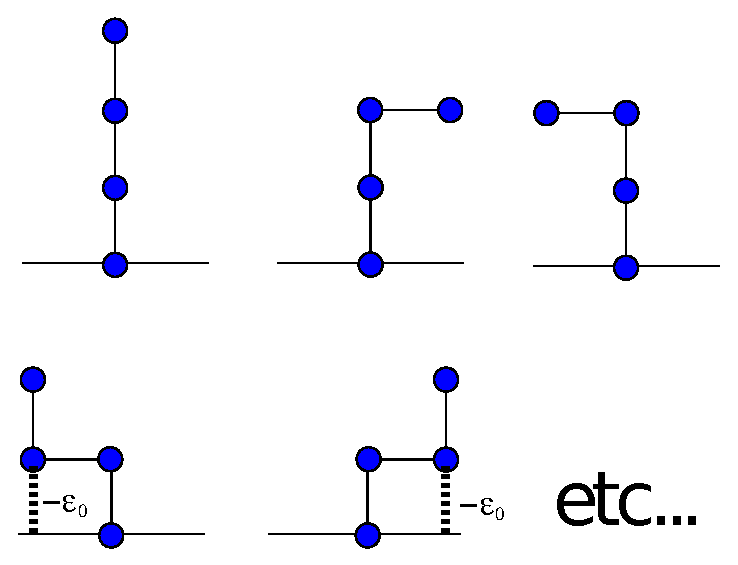
\includegraphics[width=0.4\textwidth,height=!]{molsurf}\par
\bigskip
\caption{
Several configurations of our model for a flexible molecule covalently linked to a surface.
The top row shows 3 configurations that have no favorable surface interactions.
The bottom row shows 2 configurations that have 1 favorable surface interaction.
These 5 configurations are only examples of the possible configurations
with 0, 1, or 2 surface interactions.
\label{fig:model}}
\end{figure}

\smallskip\subp
State whether these molecules are distinguishable or indistinguishable.

\smallskip\subp
Find the degeneracies for the states with 
0 surface interactions ($g_{0}$),
1 surface interaction ($g_{1}$),
and 2 surface interactions ($g_{2}$).

\smallskip\subp
Solve for the single-molecule partition function $q$ 
and the partition function $Q$ for this system using
the degeneracies and the appropriate Boltzmann weights.

\smallskip\subp
Find the Helmholtz free energy, the average energy $\left< E \right>$,
and the entropy $S$ of the system of $N$ molecules.

\smallskip\subp
Evaluate the limit of the average energy $\left< E \right>$
and the entropy $S$ as $T \rightarrow 0$.

\smallskip\subp
Evaluate the limit of the average energy $\left< E \right>$
and the entropy $S$ as $T \rightarrow \infty$.

\smallskip\subp
Explain how the average molecular height will change with temperature.

\bigskip\bigskip
\problem{12}
A plasma or ionized gas may be viewed as a mixture of positive and negative charges.
We consider as our model system a 2-D plasma
(This also happens to be an appropriate model for the motion of
parallel line vortices in an incompressible non-viscous fluid).
A simplified model for 2-D plasma contains
$N$ positive particles with charge density $e_i=e$
and $N$ negative particles with charge density $e_i = -e$ confined in a
two-dimensional ``volume'' $V$. The interaction energy for a given configuration is
$ H = -2\sum_{i<j} e_i e_j K_0\left[a ({\bf r}_i - {\bf r}_j)\right] ,$
where $K_0$ is the Bessel function of imaginary argument
and $a^{-1}$ is a cutoff distance.
By applying a rather ingenious trick, Edwards and Taylor (1974) were able to
obtain an explicit expression for the micro-canonical ensemble
partition function for this model.
Their result reads
$$ \Omega(N, V, U) = \frac{(Va^2)^{2N}}{(2N)!} \int_{-\infty}^{\infty} 
\exp\left[\frac{Va^2}{4\pi} \Big(\img z\epsilon + (1+\img z)\ln(1 + \img z) - \img z\Big) \right] {\rm d}z\,,$$
where $\epsilon \equiv U/(Ne^2)$ and $z$ are dimensionless,
and $\img$ is the imaginary unit.
Note, for this system, it is possible that $U$ is negative,
since two oppositely charged particle in close contact may contribute
a large negative value to the energy.

\smallskip\subp
In the thermodynamic limit, $V \to \infty$,
the partition function is dominated by the saddle point in the integrand.
Apply the steepest descent method, find the saddle point $z^*$,
and compute the partition by using the contribution from the saddle point alone.

\smallskip\subp
Compute the entropy $S(N,V,U)$ using the partition function.
Show that your result is thermodynamically admissible:
entropy $S$ (i) is extensive,
(ii) is a convex function of volume $V$,
and (iii) is a convex function of energy $U$.
Note: convexity $=$ negative curvature.

\smallskip\subp
Derive the equation of state for pressure, i.e., find $P=P(N,V,T)$.

\smallskip\subp
Write down an expression for the inverse temperature $1/T$.
What unusual behavior of temperature can be identified for $U > U_m = 0$?
What is the range of temperatures, for $-\infty < U < \infty$?
Plot the energetic contribution to entropy,
$$ \frac{1}{Va^2 \kB} \left[S - 2N\kB \ln\left(\frac{Va^2\ee}{2N}\right)\right], $$
against $\epsilon=U/(Ne^2)$ for $-1 < \epsilon < 1$.
\hfil\break
\strut\hfil\break
{\sl {\bf FYI:} The unusual behavior arises because the phase space is
bounded for 2-D plasmas and for vortex fluids,
and was first noted by Onsager in 1949
in a famous study of statistical theory on turbulent flow.
It can be visualized by using computer simulations (Fig.~\ref{fig:plasma}) which,
under proper condition, lead to spatial aggregation of particles with equal-sign charges.
The critical energy scale $U_m$ is $-0.4 Ne^2$ for the true plasmas,
which has no long-wavelength cutoff $a^{-1}$.
}

\begin{figure}[h]\centering
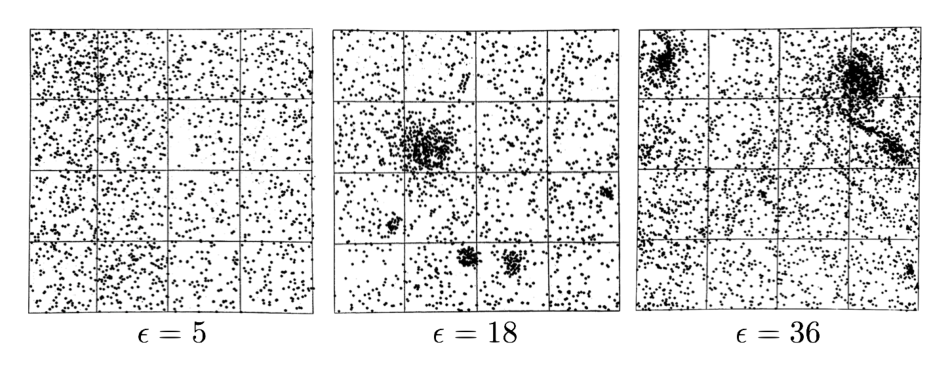
\includegraphics[width=0.618\textwidth,height=!]{plasma}
\caption{
Simulation snapshots for two dimensional plasmas.
Only positive charges are shown.
\label{fig:plasma}}
\end{figure}

